% ------------------------------------------------------------------------------
% TYPO3 Version 10.4 - What's New (Italian Version)
%
% @license	Creative Commons BY-NC-SA 3.0
% @link		https://typo3.org/help/documentation/whats-new/
% @language	Italian
% ------------------------------------------------------------------------------

\section{Modifiche per integratori}
\begin{frame}[fragile]
	\frametitle{Modifiche per integratori}

	\begin{center}\huge{Capitolo 2:}\end{center}
	\begin{center}\huge{\color{typo3darkgrey}\textbf{Modifiche per integratori}}\end{center}

\end{frame}

% ------------------------------------------------------------------------------
% Feature | 89513 | Provide password recovery for backend users

\begin{frame}[fragile]
	\frametitle{Modifiche per integratori}
	\framesubtitle{Email di recupero password (1)}

	\begin{itemize}

		\item La reimpostazione della password per gli utenti di backend sono valide solo per 4 ore.\newline
			Questo limite di tempo non è configurabile.
		\item Per rafforzare la sicurezza, la funzione può essere disabilitata per gli utenti amministratori o per tutti gli utenti.
		\item Se gli utenti condividono un indirizzo e-mail, viene utilizzato un testo e-mail alternativo.
		\item Il campo TCA \texttt{be\_users.email} non deve essere impostato a \texttt{eval=email}.

		\item La funzionalità funziona solo per gli utenti che:
			\begin{itemize}
				\item hanno impostato un indirizzo email,
				\item hanno impostato una password, e
				\item non sono disabilitati/cancellati.
			\end{itemize}

	\end{itemize}

\end{frame}

% ------------------------------------------------------------------------------
% Feature | 89513 | Provide password recovery for backend users

\begin{frame}[fragile]
	\frametitle{Modifiche per integratori}
	\framesubtitle{Email di recupero password (2)}

	\begin{itemize}
		\item Le e-mail di recupero della password possono essere attivate anche dalla riga di comando.
	\end{itemize}

	\begin{figure}
		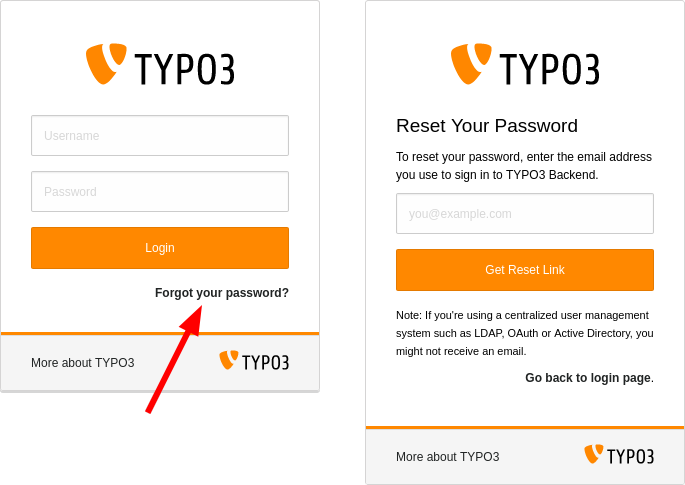
\includegraphics[width=0.9\linewidth]{ChangesForIntegrators/89513-ProvidePasswordRecoveryForBackendUsers.png}
	\end{figure}

\end{frame}

% ------------------------------------------------------------------------------
% Important | 90285 | Fresh installs without constraint for typo3fluid/fluid will get version 3.0+

\begin{frame}[fragile]
	\frametitle{Modifiche per integratori}
	\framesubtitle{Motore di template Fluid}

	\begin{itemize}
		\item Il core TYPO3 è pienamente compatibile con le versioni Fluid 2.6+ e 3.0+
		\item Le nuove installazioni senza set di dipendenze scaricheranno e installeranno Fluid versione 3.x
			(\texttt{typo3fluid/fluid:\^{}3}).
		\item Se il tuo progetto contiene template Fluid incompatibili con la versione 3.0+, esegui una delle seguenti azioni:

			\begin{itemize}
				\item Limita la versione massima: \texttt{typo3fluid/fluid:\^{}2}
				\item Aggiorna i tuoi template Fluid.
			\end{itemize}

	\end{itemize}

\end{frame}

% ------------------------------------------------------------------------------
% Important | 18079 | pages.doktype restriction for frontend queries refined

\begin{frame}[fragile]
	\frametitle{Modifiche per integratori}
	\framesubtitle{Gestione del tipo di pagina}

	\begin{itemize}
		\item La gestione interna dei tipi di pagina di TYPO3 è cambiata.
		\item L'opzione \texttt{pages.doktype} definisce un valore numerico che rappresenta il tipo,
			es. pagina standard, cartella, shortcut, link verso URL esterno, ecc.
		\item Le pagine di determinati tipi (es. cartella e cestino) sono state escluse quando il contenuto
		    è stato letto da una pagina specifica o sono stati recuperati i record.
		\item Questa limitazione è stata rimossa e sono ora possibili tipi di pagina personalizzati con un numero> 200.
		\item Agli integratori e sviluppatori che hanno utilizzato i tipi di pagina, ad es. in TypoScript, si consiglia
		    di verificare se il comportamento precedente è stato utilizzato in modo improprio e richiede ora un aggiornamento.
	\end{itemize}

\end{frame}

% ------------------------------------------------------------------------------
% Feature | 90826 | Compare backend usergroups

\begin{frame}[fragile]
	\frametitle{Modifiche per integratori}
	\framesubtitle{Modulo utenti di Backend}

	\begin{itemize}
		\item Gli integratori sono ora in grado di confrontare singoli gruppi di utenti backend.
	\end{itemize}

	\begin{figure}
		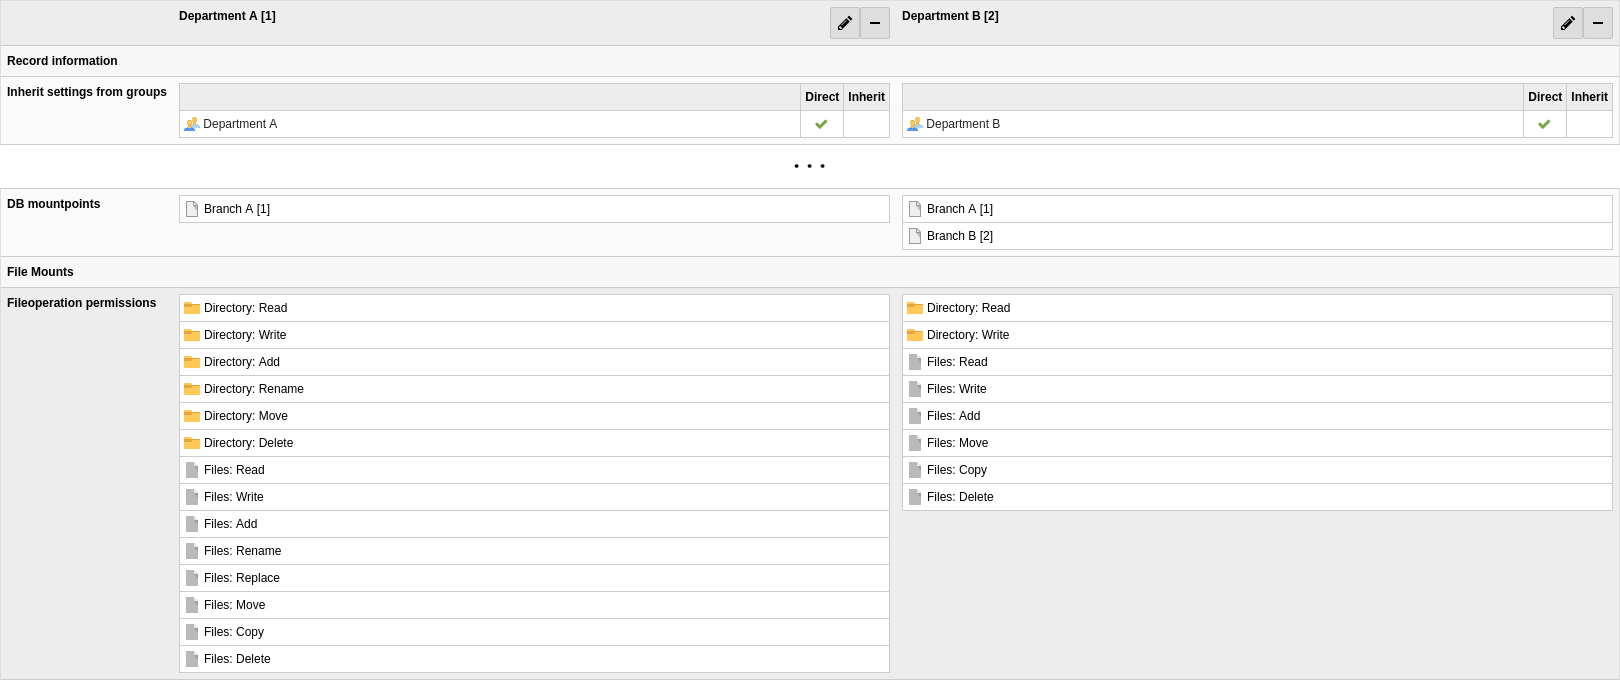
\includegraphics[width=0.9\linewidth]{ChangesForIntegrators/90826-CompareBackendUsergroups.png}
	\end{figure}

\end{frame}

% ------------------------------------------------------------------------------
% Important | 89555 | Workspace-related database records contain the proper Page ID

\begin{frame}[fragile]
	\frametitle{Modifiche per integratori}
	\framesubtitle{Workspace}

	\begin{itemize}
		\item Per molti anni, il core di TYPO3 impostava il \texttt{pid} a \texttt{-1} per i record non pubblicati.
		\item Ora TYPO3 gestisce i record con versione convalidando i seguenti tre campi:

			\begin{itemize}
				\item \texttt{t3ver\_wsid} (l'ID del workspace in cui è stato eseguito il versioning del record)
				\item \texttt{t3ver\_state} (il tipo di record versionato)
				\item \texttt{t3ver\_oid} (la versione live del record)
			\end{itemize}

		\item Perciò, \texttt{pid=-1} non è più richiesto.
		\item La procedura guidata di aggiornamento converte tutti i campi \texttt{pid} dei record versionati
			nel reale valore del \texttt{pid}.
		\item Le nuove installazioni non sono interessate da questa modifica.

	\end{itemize}

\end{frame}

% ------------------------------------------------------------------------------
% Deprecation | 91030 | Runtime-Activated Packages

\begin{frame}[fragile]
	\frametitle{Modifiche per integratori}
	\framesubtitle{Pacchetti attivati dal runtime}

	\begin{itemize}
		\item La seguente opzione di configurazione globale è stata contrassegnata \textbf{deprecata}:\newline
			\smaller
				\texttt{\$GLOBALS['TYPO3\_CONF\_VARS']['EXT']['runtimeActivatedPackages']}
			\normalsize
		\item L'uso di estensioni attivate dal runtime rallenta significativamente un'istanza di TYPO3.
		\item Si consiglia agli integratori di prendere le misure necessarie, se tali avvisi sono presenti
			nel log dei deprecati:\newline
			\begingroup
				\fontsize{8}{10}
				\texttt{Il supporto per i pacchetti attivati dal runtime verrà rimosso in TYPO3 v11.0.}
			\endgroup

	\end{itemize}

\end{frame}

% ------------------------------------------------------------------------------
